
% !TeX document-id = {a90a2b0a-e08e-44ed-850a-35793bedbf3a}
% !TeX TS-program = xelatex

% !BIB program = biber
\documentclass[handout]{beamer}
%\documentclass[compress]{beamer}
\usepackage[T1]{fontenc}
\usepackage{pifont}
\usetheme[block=fill,subsectionpage=progressbar,sectionpage=progressbar]{metropolis} 


\definecolor{Purple}{HTML}{911146}
\definecolor{Orange}{HTML}{CF4A30}

% Theme colors are derived from these two elements
\setbeamercolor{alerted text}{fg=Orange}

% ... however you can of course override styles of all elements
\setbeamercolor{frametitle}{bg=Purple}


\usepackage{wasysym}
\usepackage{etoolbox}
\usepackage[utf8]{inputenc}

\usepackage{threeparttable}
\usepackage{subcaption}

\usepackage{tikz-qtree}
\setbeamercovered{still covered={\opaqueness<1->{5}},again covered={\opaqueness<1->{100}}}


\usepackage{listings}

\lstset{
	basicstyle=\scriptsize\ttfamily,
	columns=flexible,
	breaklines=true,
	numbers=left,
	%stepsize=1,
	numberstyle=\tiny,
	backgroundcolor=\color[rgb]{0.85,0.90,1}
}



\lstnewenvironment{lstlistingoutput}{\lstset{basicstyle=\footnotesize\ttfamily,
		columns=flexible,
		breaklines=true,
		numbers=left,
		%stepsize=1,
		numberstyle=\tiny,
		backgroundcolor=\color[rgb]{.7,.7,.7}}}{}


\lstnewenvironment{lstlistingoutputtiny}{\lstset{basicstyle=\tiny\ttfamily,
		columns=flexible,
		breaklines=true,
		numbers=left,
		%stepsize=1,
		numberstyle=\tiny,
		backgroundcolor=\color[rgb]{.7,.7,.7}}}{}


\usepackage[american]{babel}
\usepackage{csquotes}
\usepackage[style=apa, backend = biber]{biblatex}
\DeclareLanguageMapping{american}{american-UoN}
\addbibresource{../literature.bib}
\renewcommand*{\bibfont}{\tiny}

\usepackage{tikz}
\usetikzlibrary{shapes,arrows,matrix}
\usepackage{multicol}

\usepackage{subcaption}

\usepackage{booktabs}
\usepackage{graphicx}

\graphicspath{{../pictures/}}

\makeatletter
\setbeamertemplate{headline}{%
	\begin{beamercolorbox}[colsep=1.5pt]{upper separation line head}
	\end{beamercolorbox}
	\begin{beamercolorbox}{section in head/foot}
		\vskip2pt\insertnavigation{\paperwidth}\vskip2pt
	\end{beamercolorbox}%
	\begin{beamercolorbox}[colsep=1.5pt]{lower separation line head}
	\end{beamercolorbox}
}
\makeatother



\setbeamercolor{section in head/foot}{fg=normal text.bg, bg=structure.fg}



\newcommand{\question}[1]{
	\begin{frame}[plain]
		\begin{columns}
			\column{.3\textwidth}
			\makebox[\columnwidth]{
				
\includegraphics[width=\columnwidth,height=\paperheight,keepaspectratio]{../pictures/mannetje.png}}
			\column{.7\textwidth}
			\large
			\textcolor{orange}{\textbf{\emph{#1}}}
		\end{columns}
\end{frame}}

\newcommand{\instruction}[1]{\emph{\textcolor{gray}{[#1]}}}


\title[Computational Communication Science 2]{\textbf{Computational Communication Science 2} \\Week 7 - Lecture\\ »Rule-based vs. Automated Text Classification«}
\author[Marthe Möller, Anne Kroon]{Marthe Möller \\ Anne Kroon \\ ~ \\ \footnotesize{a.m.moller@uva.nl, @marthemoller \\a.c.kroon@uva.nl, @annekroon} \\}
\date{May, 2022}
\institute[Digital Society Minor, University of Amsterdam]{Digital Society Minor, University of Amsterdam}


\begin{document}
	
	\begin{frame}{}
		\titlepage
	\end{frame}
	
	\begin{frame}{Today}
		\tableofcontents
	\end{frame}
	
	
	\section{Rule-based Text Classification}
	
	\begin{frame}{Text Classification} 
		
	Text classification: To assign a label to a text.
	
	For example, to distinguish between:
	\begin{itemize}
		\item newspaper articles about sports vs. economics.
		\item reliable vs. unreliable information about vaccination.
		\item webpages about holding companies vs. financing companies.
		\item positive vs. negative movie reviews.
	\end{itemize}
	
	\end{frame}
		
	\begin{frame}{Studying Flaming (Example)} 
	
	RQ: How problematic is flaming on Twitter? \\
	Bag-of-words approach:
	
	\begin{enumerate}
		\item Create a list with all the swearwords that exist.
		\item For each tweet in the dataset, use the list to count the number of swearwords	
		\item If a tweet contains X number of swearwords label it as flaming
	\end{enumerate}
	

\end{frame}


	\begin{frame}{Sentiment Analysis} 
	
	We can add nuance by creating more rules.
	
	For example, in sentiment analyses, we can include a rule telling the machine what to do in case of negation or modifiers.
	
	"This movie is really not good." \\
	"This movie is really good."
		
	\end{frame}


	\begin{frame}{Rule-based Text Classifcation} 
	
	Advantages of rule-based text classification:
	\begin{itemize}
		\item Simple and therefore transparent
		\item Cheap
	\end{itemize}
	
	Challenges of rule-based text classification:
	\begin{itemize}
		\item Not a suitable way to anayze latent or abstract variables 
		\item You must know all the categories beforehand
		\item You must know and be able to express all the rules
	\end{itemize}

	\end{frame}


\begin{frame}{From Rule-based to Automated}

	When it is easy for humans to decide to what class a text belongs, but we struggle to translate our decision process into straight-forward rules, we are likely to be better of using a form of automated text classification: Supervised Machine Learning.
	
\end{frame}


	
	\section{SML}
	
	
	\begin{frame}{What is SML?}
		
		\begin{center}
			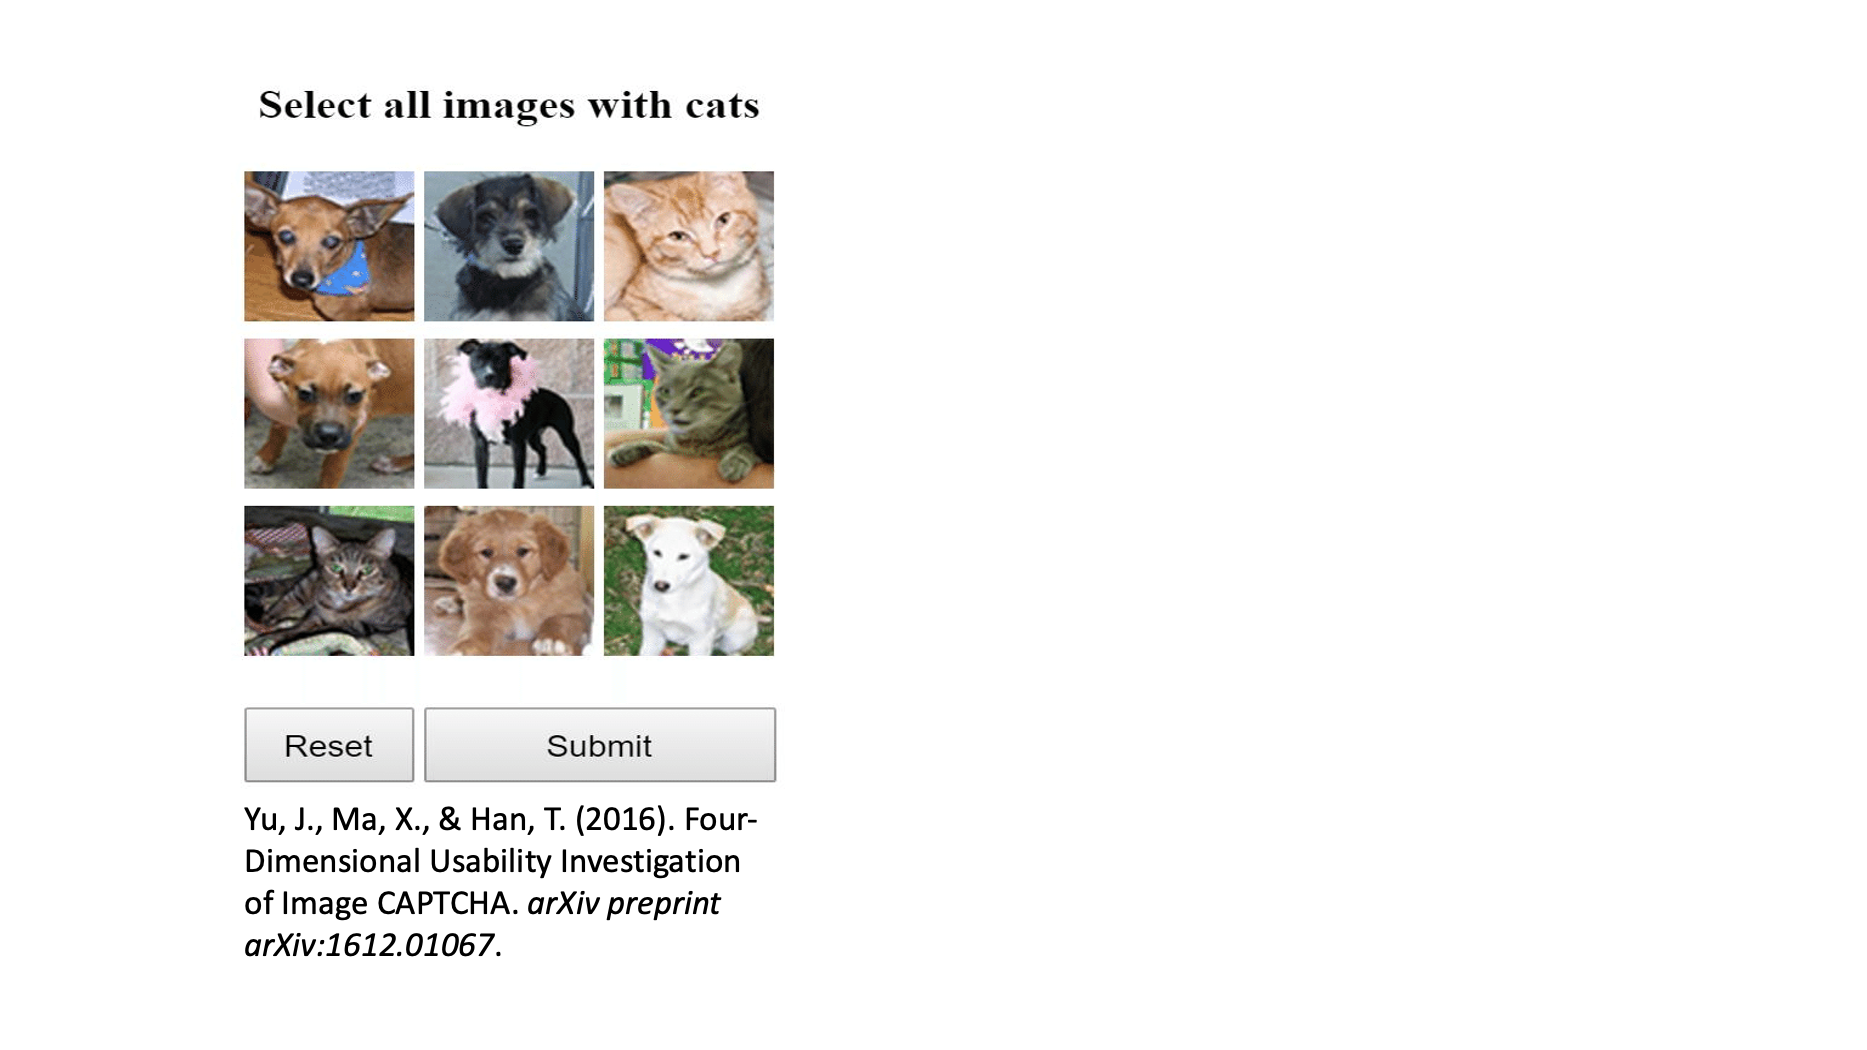
\includegraphics[width=4cm, height=7cm]{../pictures/CAPTCHA.png} 
		\end{center}
		
		
	\end{frame}
	
	
	\begin{frame}{What is SML?}
		
		\begin{center}
			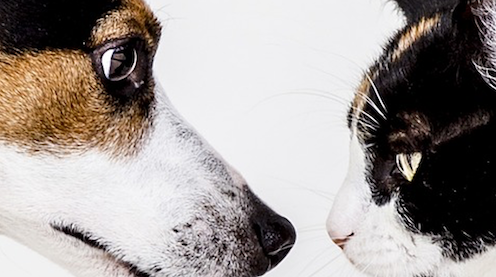
\includegraphics{../pictures/dogvscat.png}
		\end{center}
		
		\begin{tiny}
			Read more about this project in: 
			\fullcite{sermanet_overfeat_2014} 
		\end{tiny}
		
		
	
	\end{frame}
	


\begin{frame}{What is ML?} 
	
Machine Learning: “a type of artificial intelligence in which computers use huge amounts of data to learn how to do tasks rather than being programmed to do them.” \\\
	
	\begin{tiny}
		Oxford Dictionary
	\end{tiny}

\end{frame}





	\begin{frame}{What is SML?} 
		
		Supervised Machine Learning (SML): “A form of machine learning, where we aim to predict a variable that, for a least part of our data is known.” \\\
		
		\begin{tiny}
			\fullcite{van_atteveldt_computational_2022} 
		\end{tiny}
		
	
	\end{frame}
	
	
	\begin{frame}{What is SML?} 
		
		“The goal of Supervised Machine Learning: estimate a model based on some data, and then use the model to predict the expected outcome for some new cases, for which we do not know the outcome yet.” \\\
		
		\begin{tiny}
			\fullcite{van_atteveldt_computational_2022} 
		\end{tiny}
		
		
		
	\end{frame}
	
	\begin{frame}{What is SML?} 
		
		Machine Learning has a lot of similarities to regression analysis!
		

		
	\end{frame}
	
	
	\section{The principles behind SML}
	
	\begin{frame}{The principles behind SML} 
		
		\(y = constant + b_1 * x_1 + b_2 * x_2\) 
		
		\(x_1\) = bark? (0= no, 1 = yes) \\\
		\(x_2\) = tail? (0 = no, 1 = yes) \\\
		\(y\) = Is this a dog? ( 0 = definitely no, 1 = definitely yes)

	\end{frame}
	
	
	\begin{frame}{The principles behind SML} 
		
		\(y = constant + b_1 * x_1 + b_2 * x_2\) \\\
		
		\(y = 0 + 0.8 * x_1 + 0.2 * x_2\) \\\
		
		
	
		
	\end{frame}
	
	\begin{frame}{The principles behind SML} 
		
		\(y = 0 + 08 * 1 + 0.2 * 0\) \\\
		
		\(0.8 = 0 + 0.8 * 1 + 0.2 * 0\) \\\
		
		
	\end{frame}
	
	\begin{frame}{The principles behind SML} 
		
		\(0.8 = 0 + 0.8 * 1 + 0.2 * 0\) \\\
		
		Classification: a predictive modeling problem where a class label is predicted for a given example of input data. 
		
		
	
	\end{frame}
	
	
	\begin{frame}{The principles behind SML}
		
		\begin{center}
			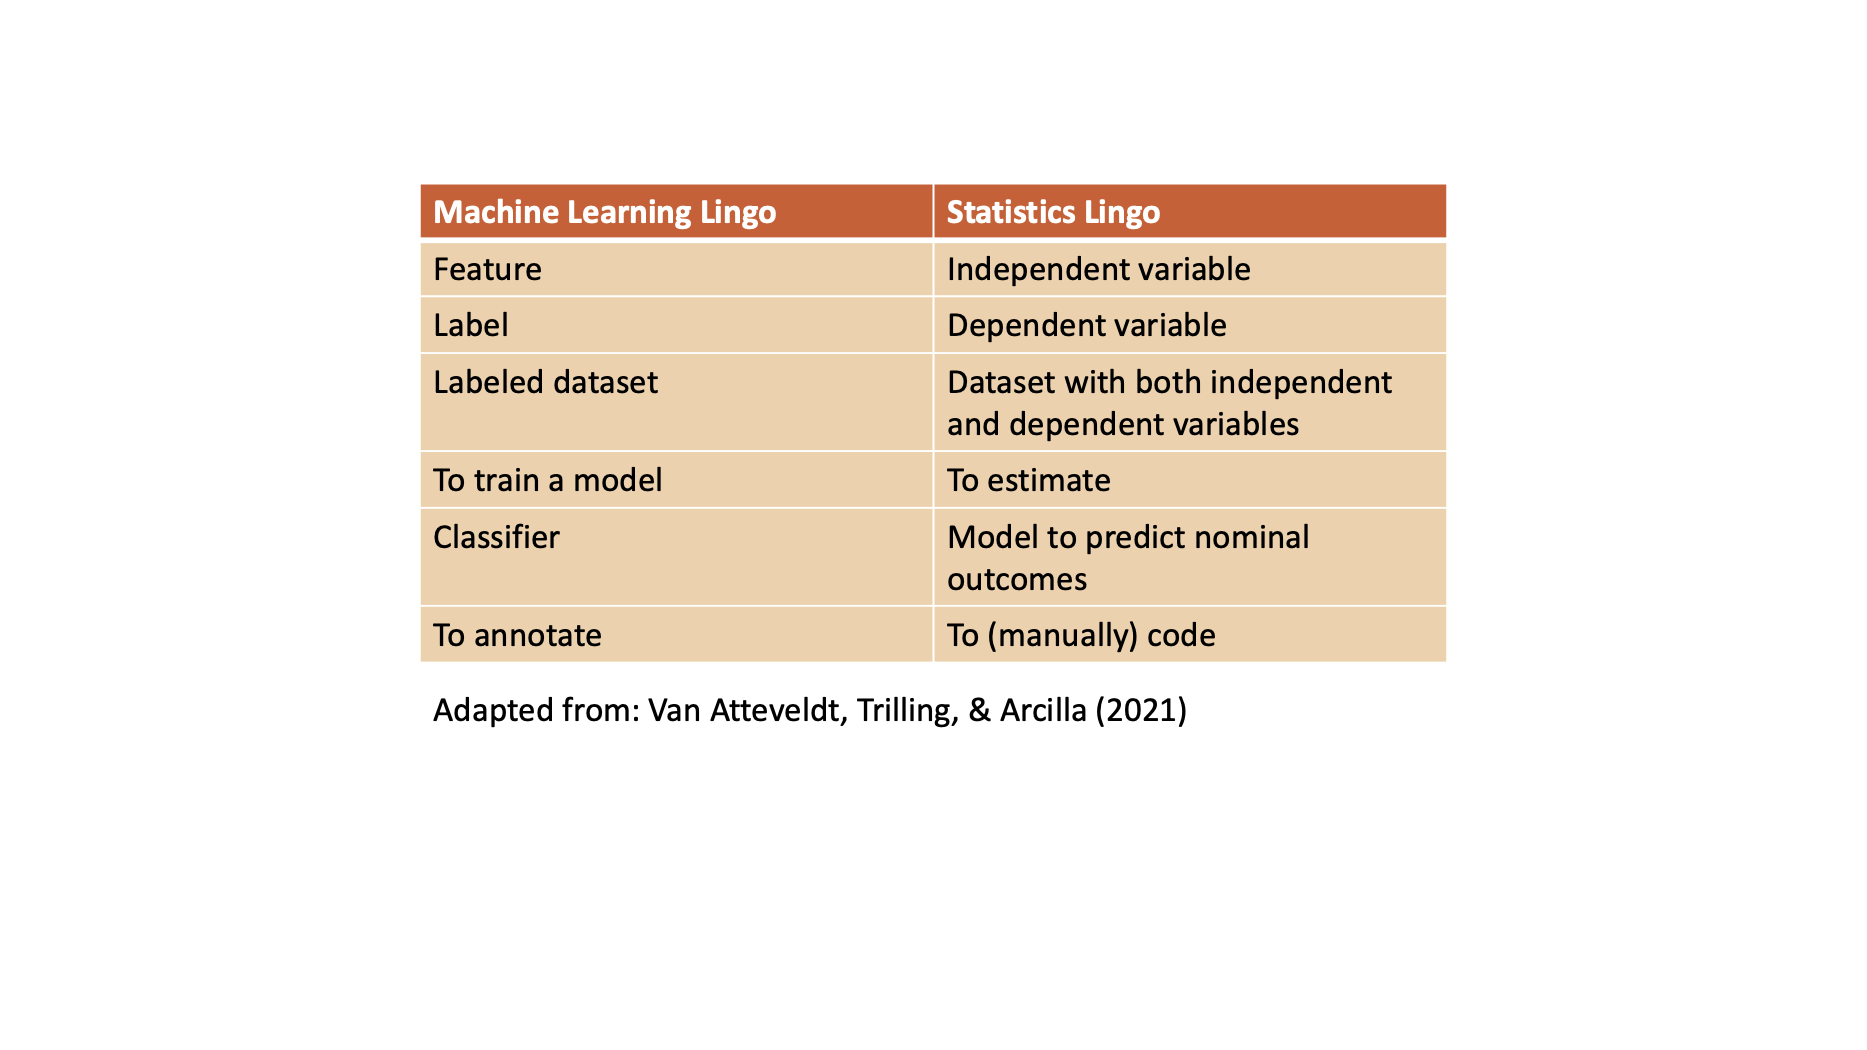
\includegraphics[width=\linewidth,height=\textheight,keepaspectratio]{../pictures/MLlingo.png} \\\
		\end{center}
			
	\end{frame}
	
	
	\begin{frame}{The principles behind SML} 
		
		Machine Learning: using a (regression) formula to predict a label. \\\
		
		Traditional usage of formulas in CS: to explain \\\
		
		Usage of formulas in ML: to predict \\\
		
		
	\end{frame}
	
	
	
	\begin{frame}{Zooming out} 
		
		We talked about:
		\begin{itemize}
			\item Rule-based Text Classification
			\item Automated Text Classification: SML
			\item The principles behind SML \\\
		\end{itemize}
		
		Next, we will talk about:
		\begin{itemize}
			\item Some commonly used SML models
		\end{itemize}
		
	\end{frame}
	
	
	\section{SML models}
	
	\begin{frame}{SML step by step}
		
		\begin{center}
			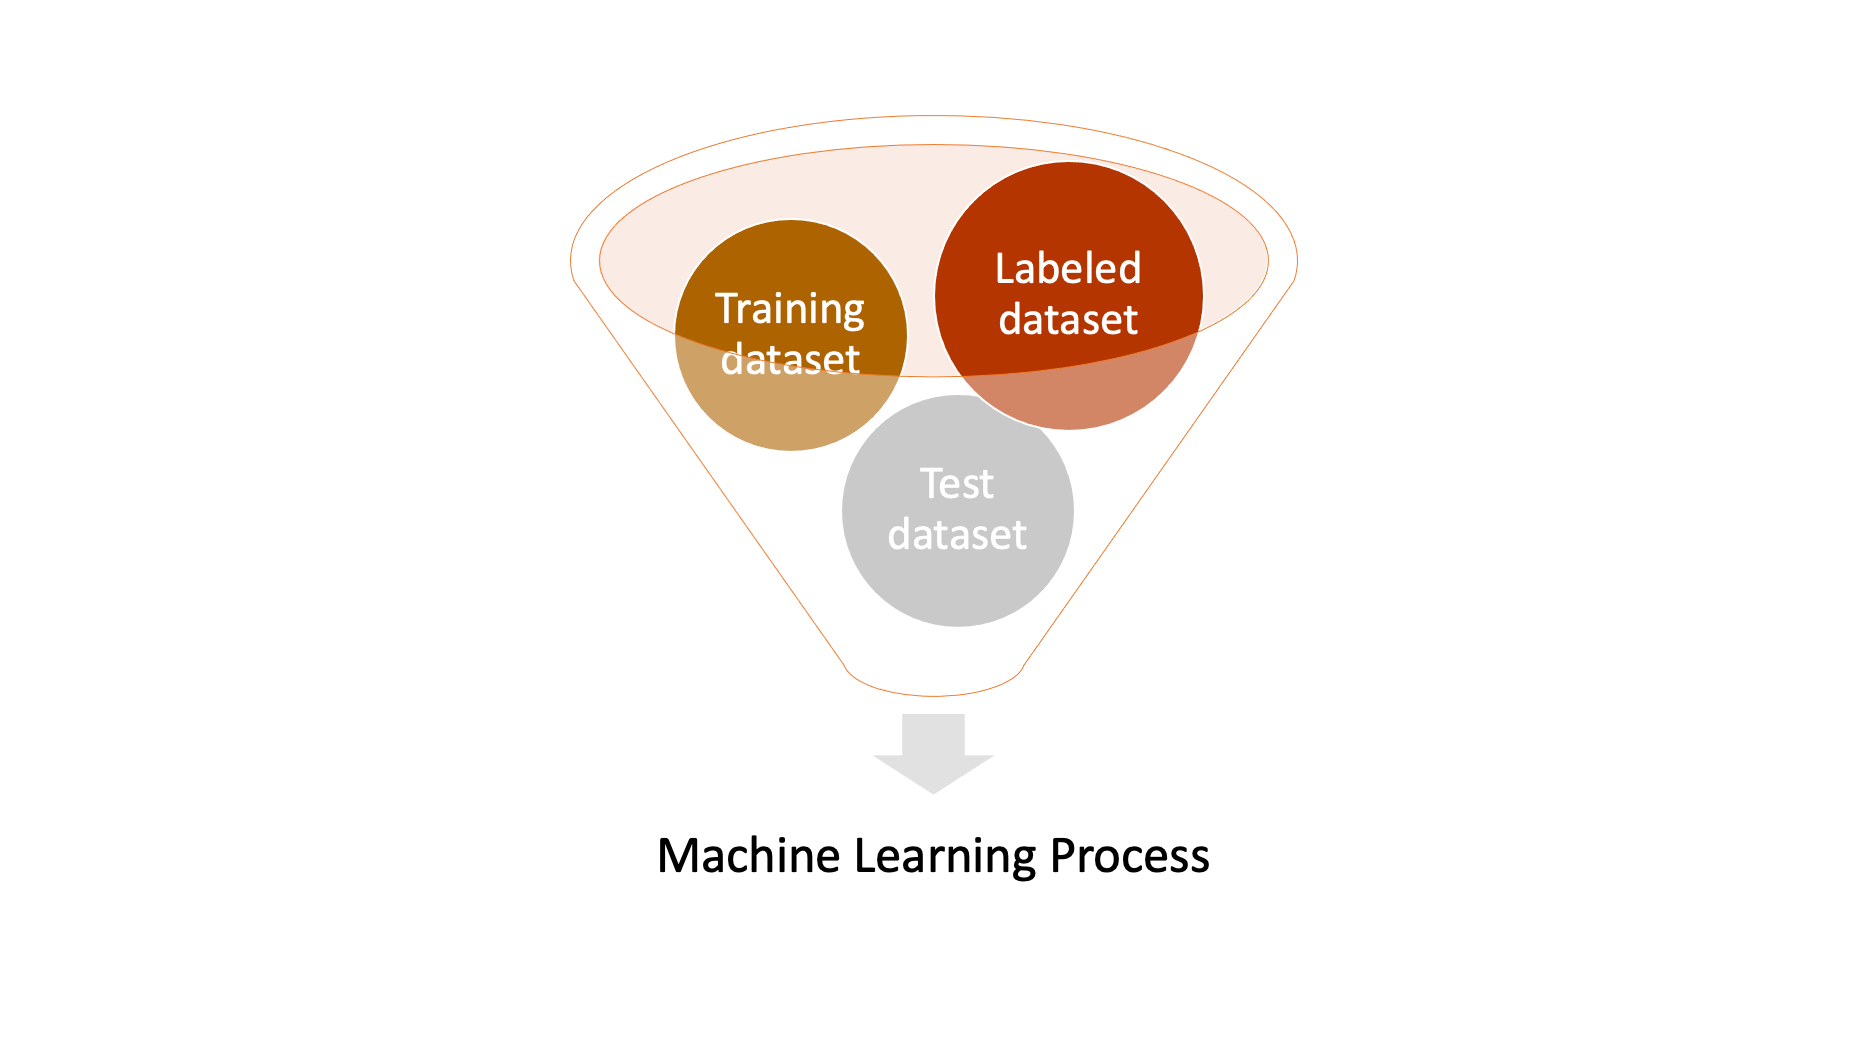
\includegraphics[width=\linewidth,height=\textheight,keepaspectratio]{../pictures/MLingredients.png} \\\
		\end{center}

		
	\end{frame}
	
	
	\begin{frame}{SML step by step}
		
		\begin{center}
			
\includegraphics[width=\linewidth,height=\textheight,keepaspectratio]{../pictures/MLprocess.png} \\\
		\end{center}
	
		Let's have a look at some commonly used ML models.
		
		

		
	\end{frame}
	

\begin{frame}{Regression}
	
	\begin{center}
		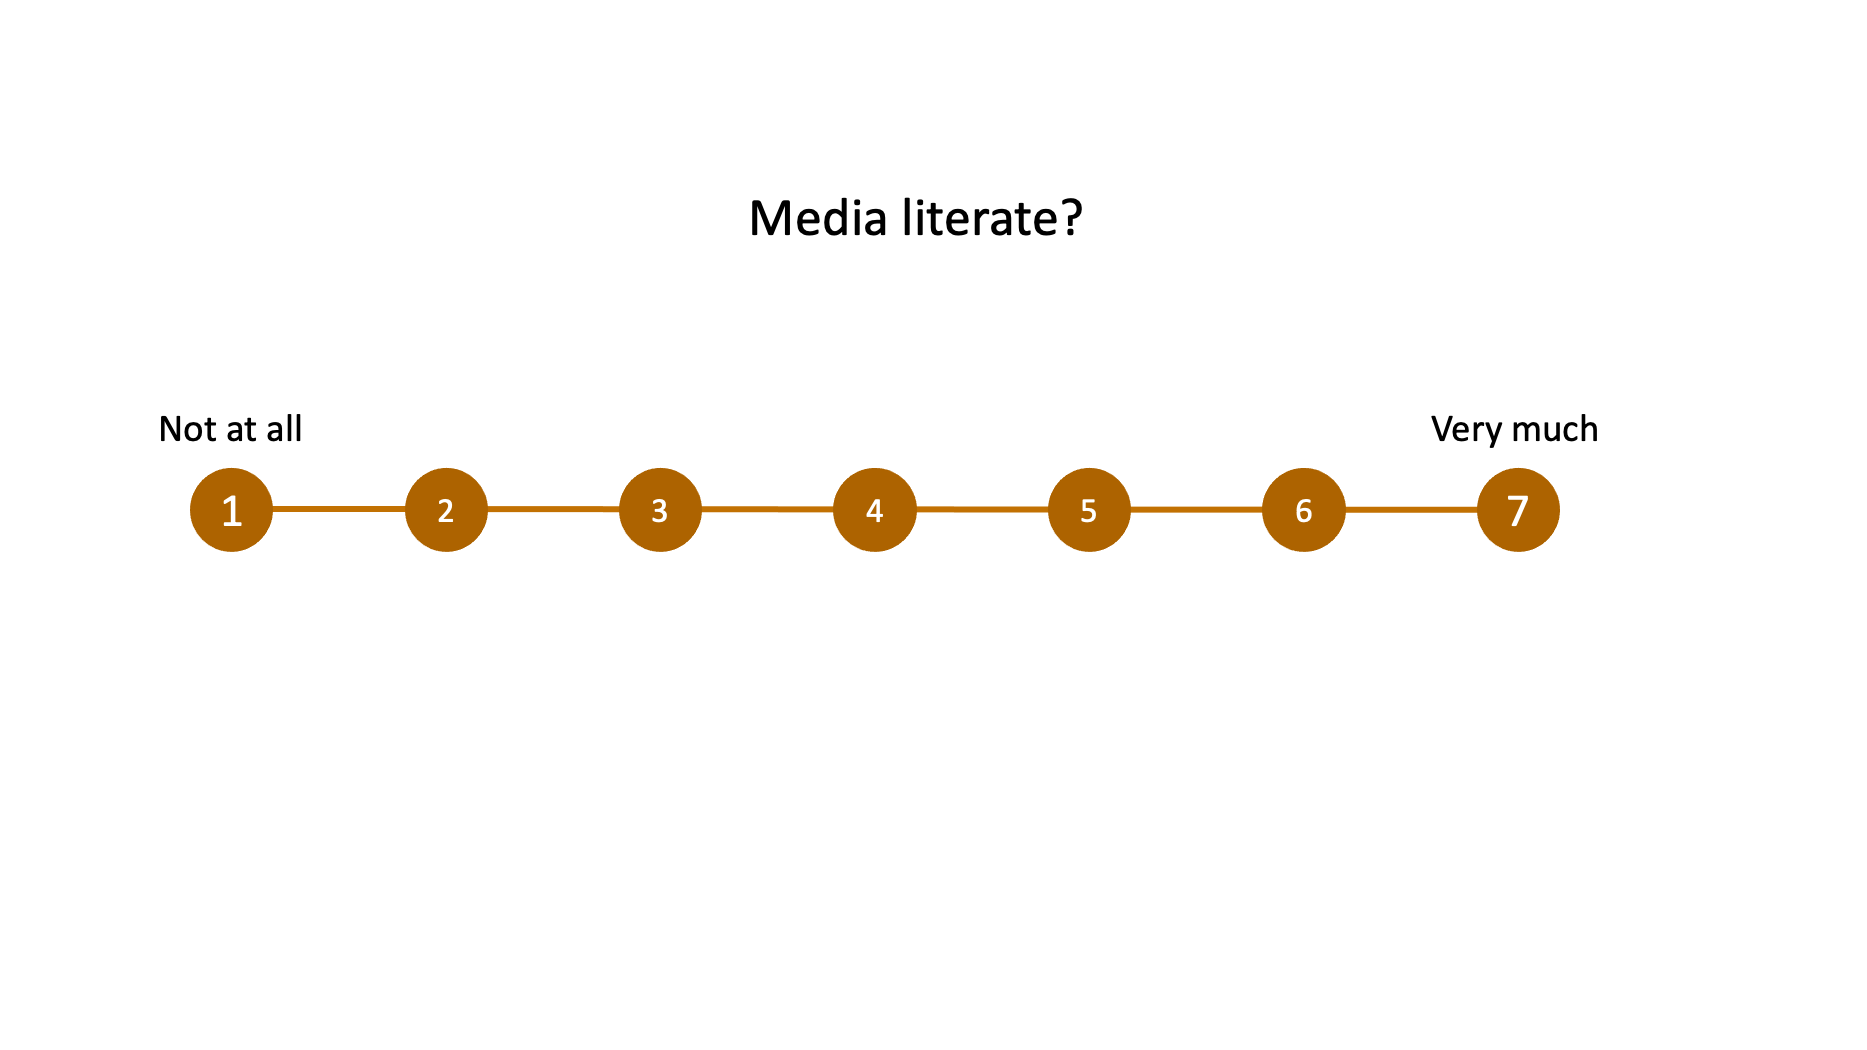
\includegraphics[width=\linewidth,height=\textheight,keepaspectratio]{../pictures/medialiteracyscale.png} \\\
	\end{center}
	
	

	
	
\end{frame}



\begin{frame}{Logistic Regression}
	
	\begin{center}
		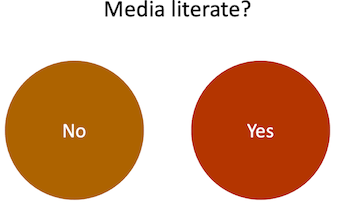
\includegraphics{../pictures/medialiteracydummy.png} \\\
	\end{center}
	

	
\end{frame}


\begin{frame}{Logistic Regression}
	
	\begin{center}
		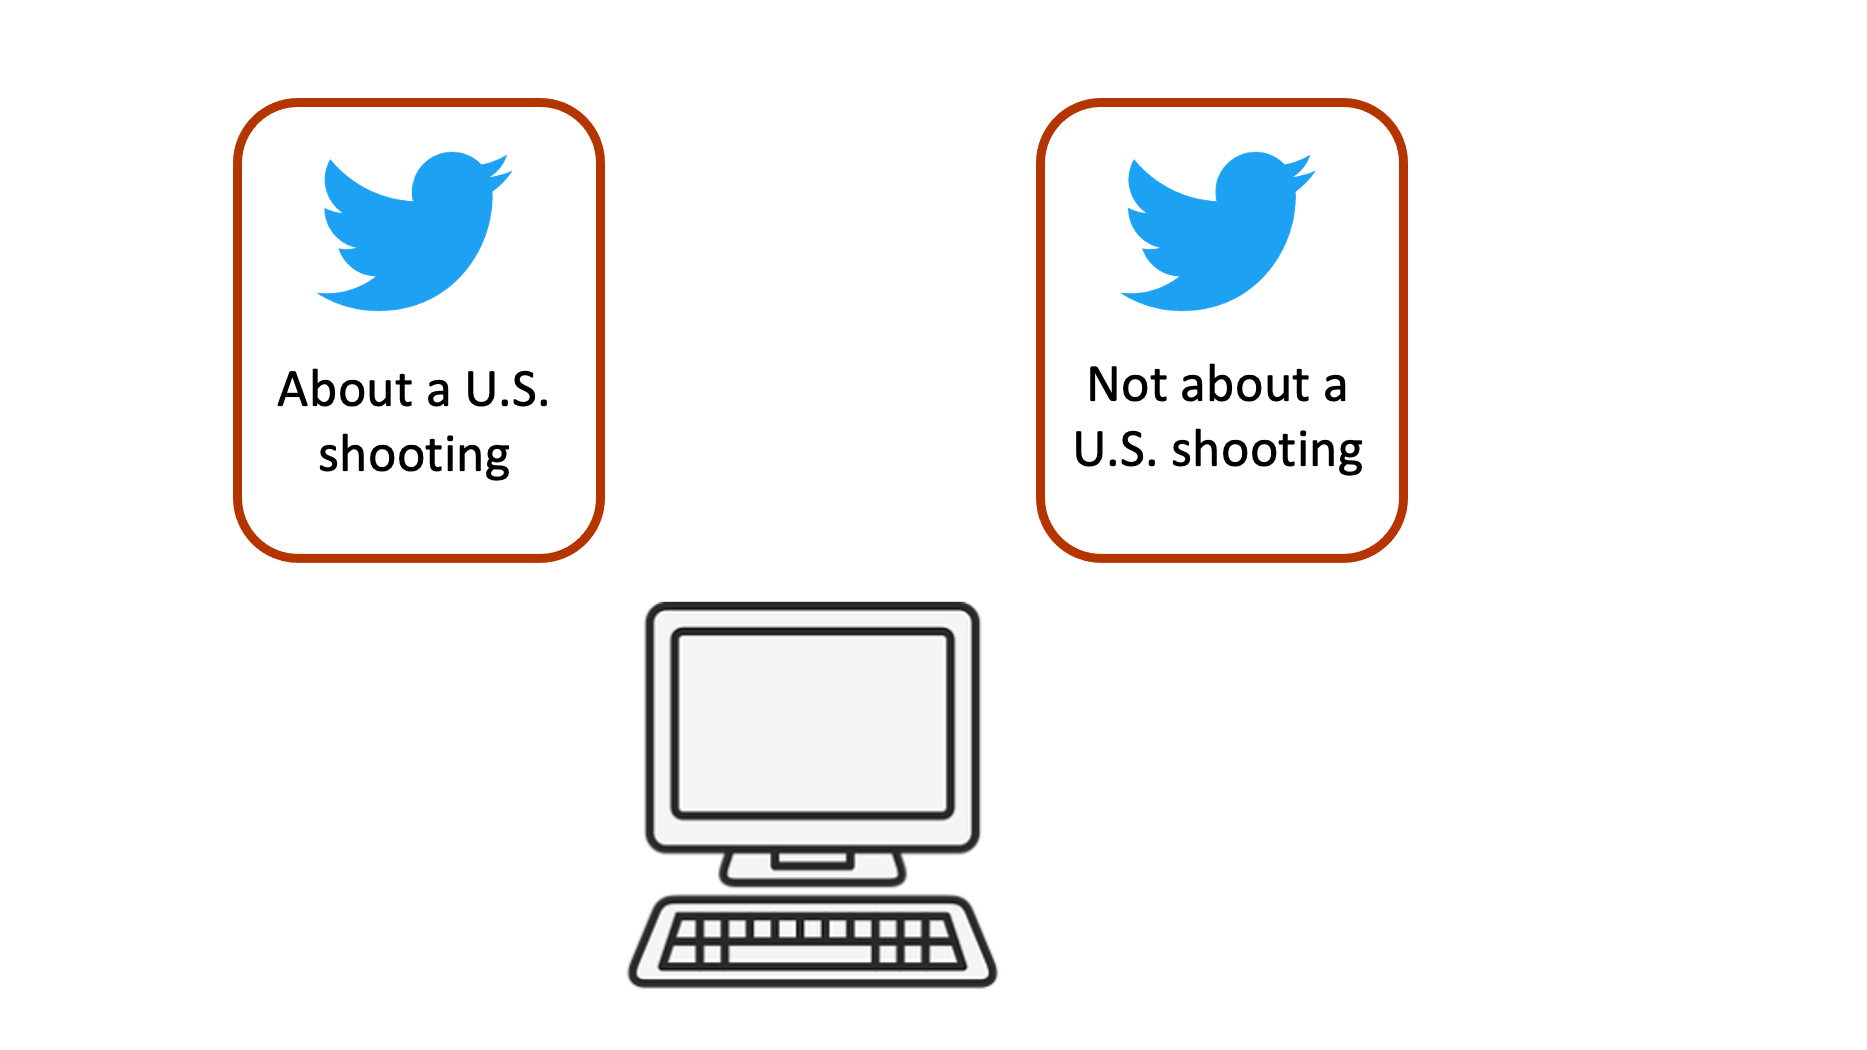
\includegraphics{../pictures/Zhangetal_1.png} \\\
	\end{center}
	
	\begin{tiny}
		\fullcite{zhang_whose_2019} 
	\end{tiny}
\end{frame}


\begin{frame}{Logistic Regression}
	
	\begin{center}
		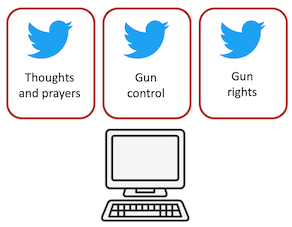
\includegraphics{../pictures/Zhangetal_2.png} \\\
	\end{center}
	
	\begin{tiny}
		\fullcite{zhang_whose_2019} 
	\end{tiny}
	

	
\end{frame}


\begin{frame}{Logistic Regression}
	
	\begin{center}
		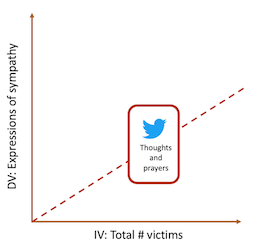
\includegraphics{../pictures/Zhangetal_3.png} \\\
	\end{center}
	
	\begin{tiny}
		\fullcite{zhang_whose_2019} 
	\end{tiny}
	

	
\end{frame}


\begin{frame}[fragile]{What does this look like in code?}

First, we need to read in the ingredients we need for SML.
\begin{lstlisting}
import csv
from sklearn.model_selection import train_test_split

tweets = []
labels = []

with open(file) as fi:
     data = csv.reader(fi, delimiter='\t')
     for row in data:
          tweets.append(row[0])
          labels.append(row[1])

tweets_train, tweets_test, y_train, y_test = train_test_split(tweets, labels, test_size=0.2, random_state=42)
\end{lstlisting}
	
Where file is some file containg tweets (column 0) and their labels (column 1).
	
\end{frame}




\begin{frame}[fragile]{What does this look like in code?}
	
Second, vectorize the texts that need to be labeled: 

\begin{lstlisting}
from sklearn.feature_extraction.text import (TfidfVectorizer)

tfidfvectorizer = TfidfVectorizer(stop_words="english")
X_train = tfidfvectorizer.fit_transform(tweets_train)
X_test = tfidfvectorizer.transform(tweets_test)

\end{lstlisting}

Where tweets\_train and tweets\_test are two lists with tweets (strings)
	
\end{frame}


\begin{frame}[fragile]{What does this look like in code?}
	
Next, I train my machine and test it: 
	
\begin{lstlisting}
from sklearn.linear_model import (LogisticRegression)

logres = LogisticRegression()
logres.fit(X_train, labels_train)
y_pred = logres.predict(X_test)
\end{lstlisting}
	
\end{frame}


\begin{frame}[fragile]{What does this look like in code?}
	
To train a model based on a tf-idf vectorizer and Log Regression:
	
\begin{lstlisting}
from sklearn.feature_extraction.text import (TfidfVectorizer)
from sklearn.linear_model import (LogisticRegression)

tfidfvectorizer = TfidfVectorizer(stop_words="english")
X_train = tfidfvectorizer.fit_transform(tweets_train)
X_test = tfidfvectorizer.transform(tweets_test)

logres = LogisticRegression()
logres.fit(X_train, labels_train)
y_pred = logres.predict(X_test)
\end{lstlisting}
	
\end{frame}



\begin{frame}{Na\"{\i}ve Bayes}
	
	\begin{center}
		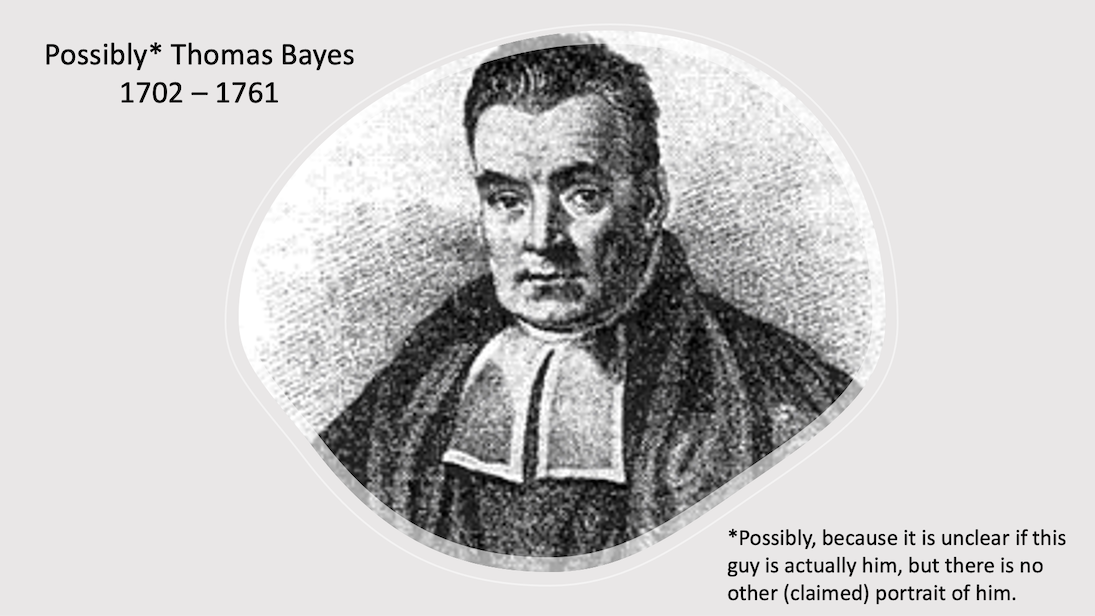
\includegraphics[width=\linewidth,height=\textheight,keepaspectratio]{../pictures/ThomasBayes.png} \\\
	\end{center}
	

\end{frame}



\begin{frame}{Na\"{\i}ve Bayes}
	
	$ P(\rm{A} \mid \rm{B}) = \frac{P(\rm{B} \mid \rm{A}) \cdot P(\rm{A})}{P(\rm{B})} $
	
	Mathematicians’ language for: the probability of A if B is the case/present/true. 
	
	$ P(\rm{label} \mid \rm{features}) = \frac{P(\rm{features} \mid \rm{label}) \cdot P(\rm{label})}{P(\rm{features})} $
	
	


\end{frame}


\begin{frame}[fragile]{What does this look like in code?}
	
Let's also train a model based on a count vectorizer and Naïve Bayes:
	
\begin{lstlisting}
from sklearn.feature_extraction.text import (CountVectorizer)
from sklearn.naive_bayes import MultinomialNBB

countvectorizer = CountVectorizer(stop_words="english")
X_train = countvectorizer.fit_transform(texts_train)
X_test = countvectorizer.transform(texts_test)

nb = MultinomialNB()
nb.fit(X_train, labels_train)
y_pred = nb.predict(X_test)
\end{lstlisting}
	
\end{frame}




\begin{frame}{Support Vector Machines}
	
	SVMs aim to find a hyperplane in an \(N\)-dimensional pace that distinctly classifies the datapoints.
	
	The best hyperplane is the one that has the maximum margin (distance) between the datapoints of both classes.
	
	\begin{center}
		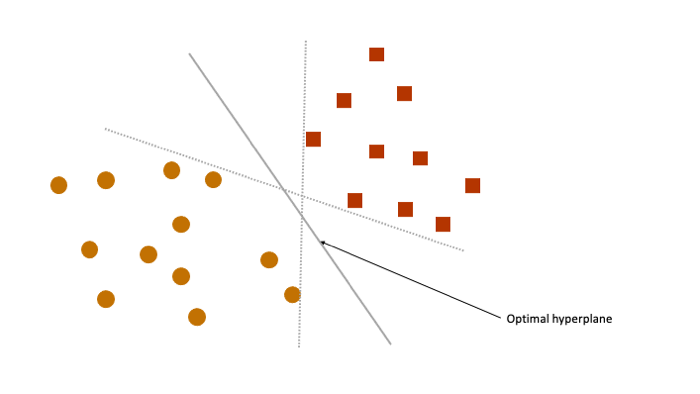
\includegraphics[width=\linewidth,height=0.5\textheight,keepaspectratio]{../pictures/optimal_hyperplane.png} \\\
	\end{center}
	
\end{frame}

\begin{frame}{Support Vector Machines}
	
	\begin{center}
		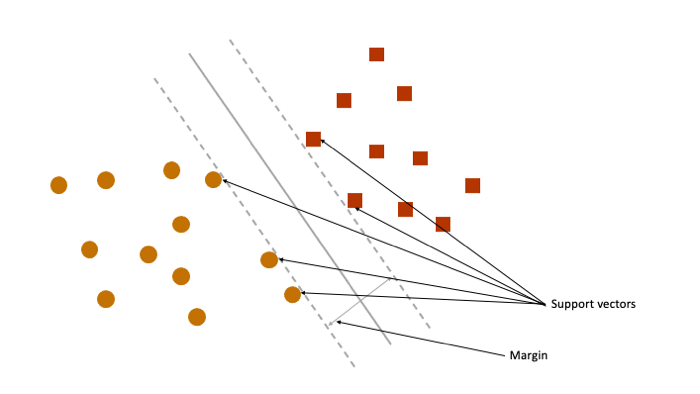
\includegraphics[width=\linewidth,height=\textheight,keepaspectratio]{../pictures/SVM.png} \\\
	\end{center}
	
\end{frame}


\begin{frame}{Decision Trees and Random Forests}
	
	\begin{center}
		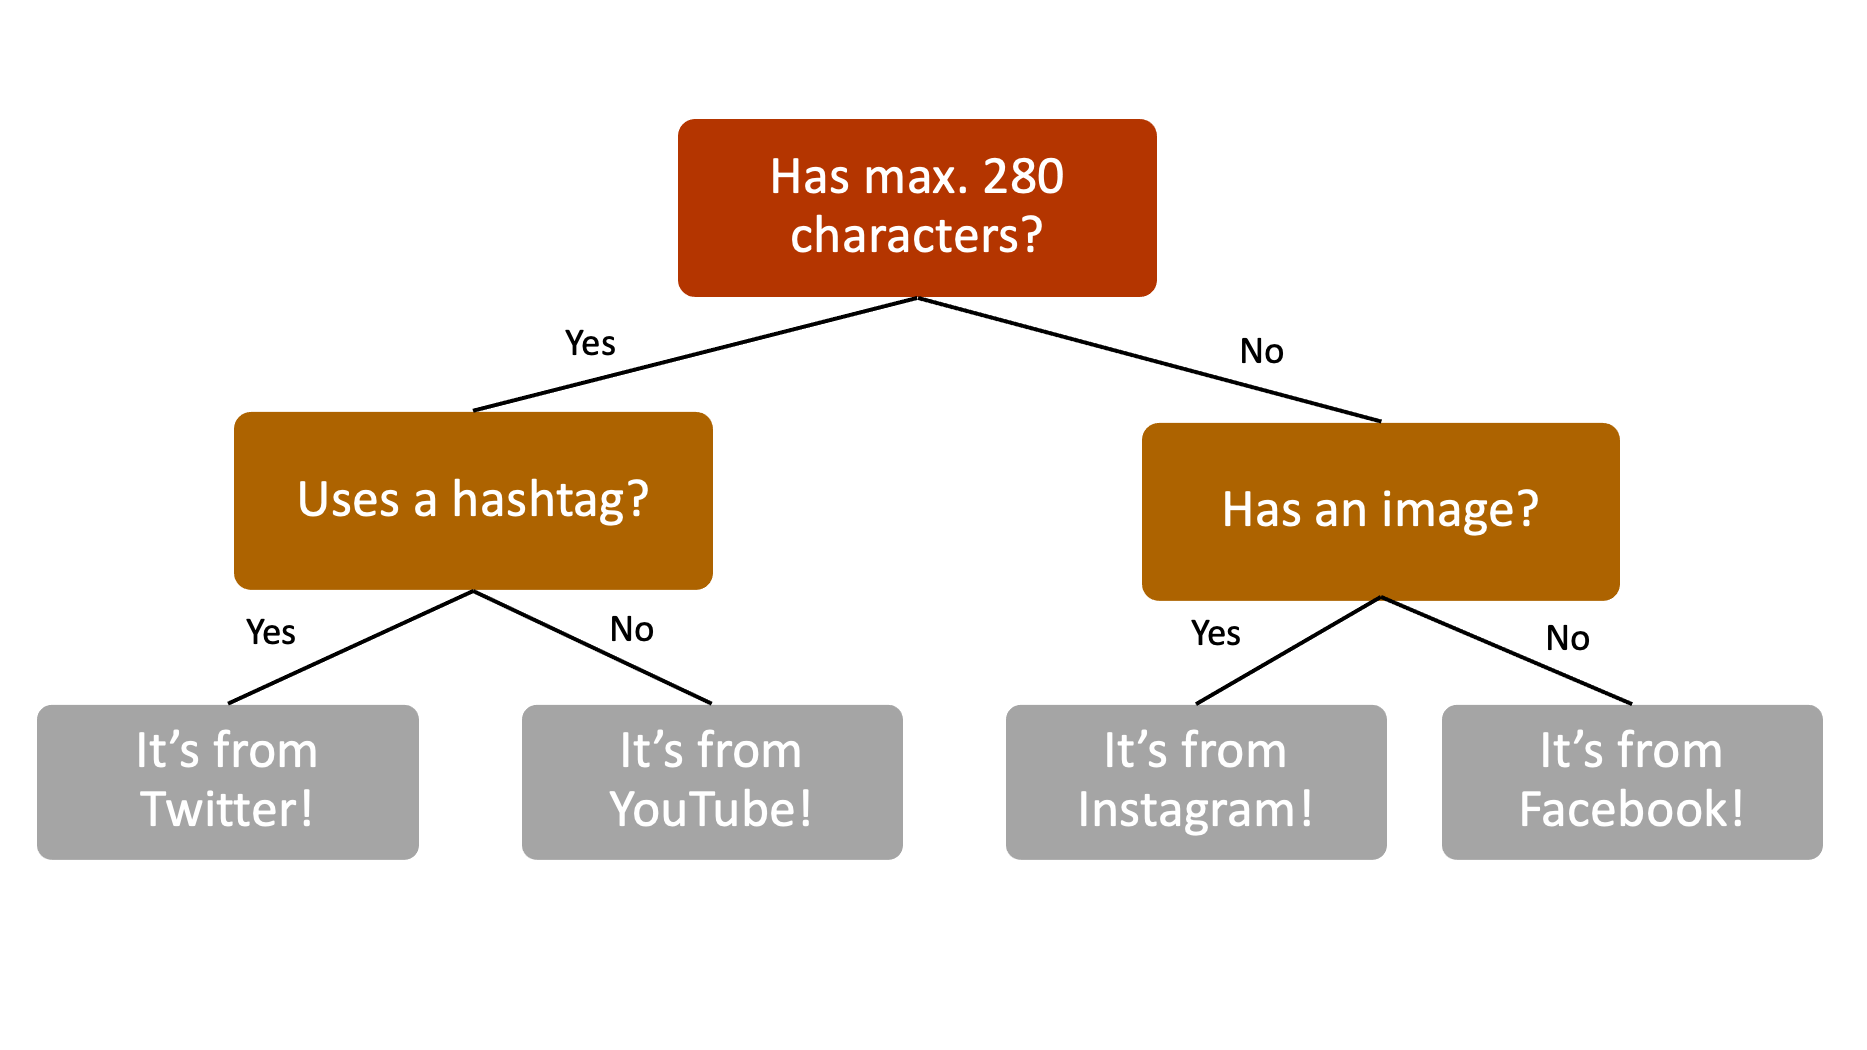
\includegraphics[width=\linewidth,height=\textheight,keepaspectratio]{../pictures/decisiontree.png} \\\
	\end{center}
	

	
\end{frame}



\begin{frame}{Decision Trees and Random Forests} 
	
	Advantages of decision trees:
	\begin{itemize}
		\item Transparency
		\item Suitable for non-linear relationships \\\
	\end{itemize}
	
	Disadvatanges of decision trees:
	\begin{itemize}
		\item Loss of nuance due to yes/no-design
		\item Cannot correct early mistakes
		\item Prone to overfitting
	\end{itemize}
	
	
\end{frame}


\begin{frame}{Decision Trees and Random Forests}
	
	\begin{center}
		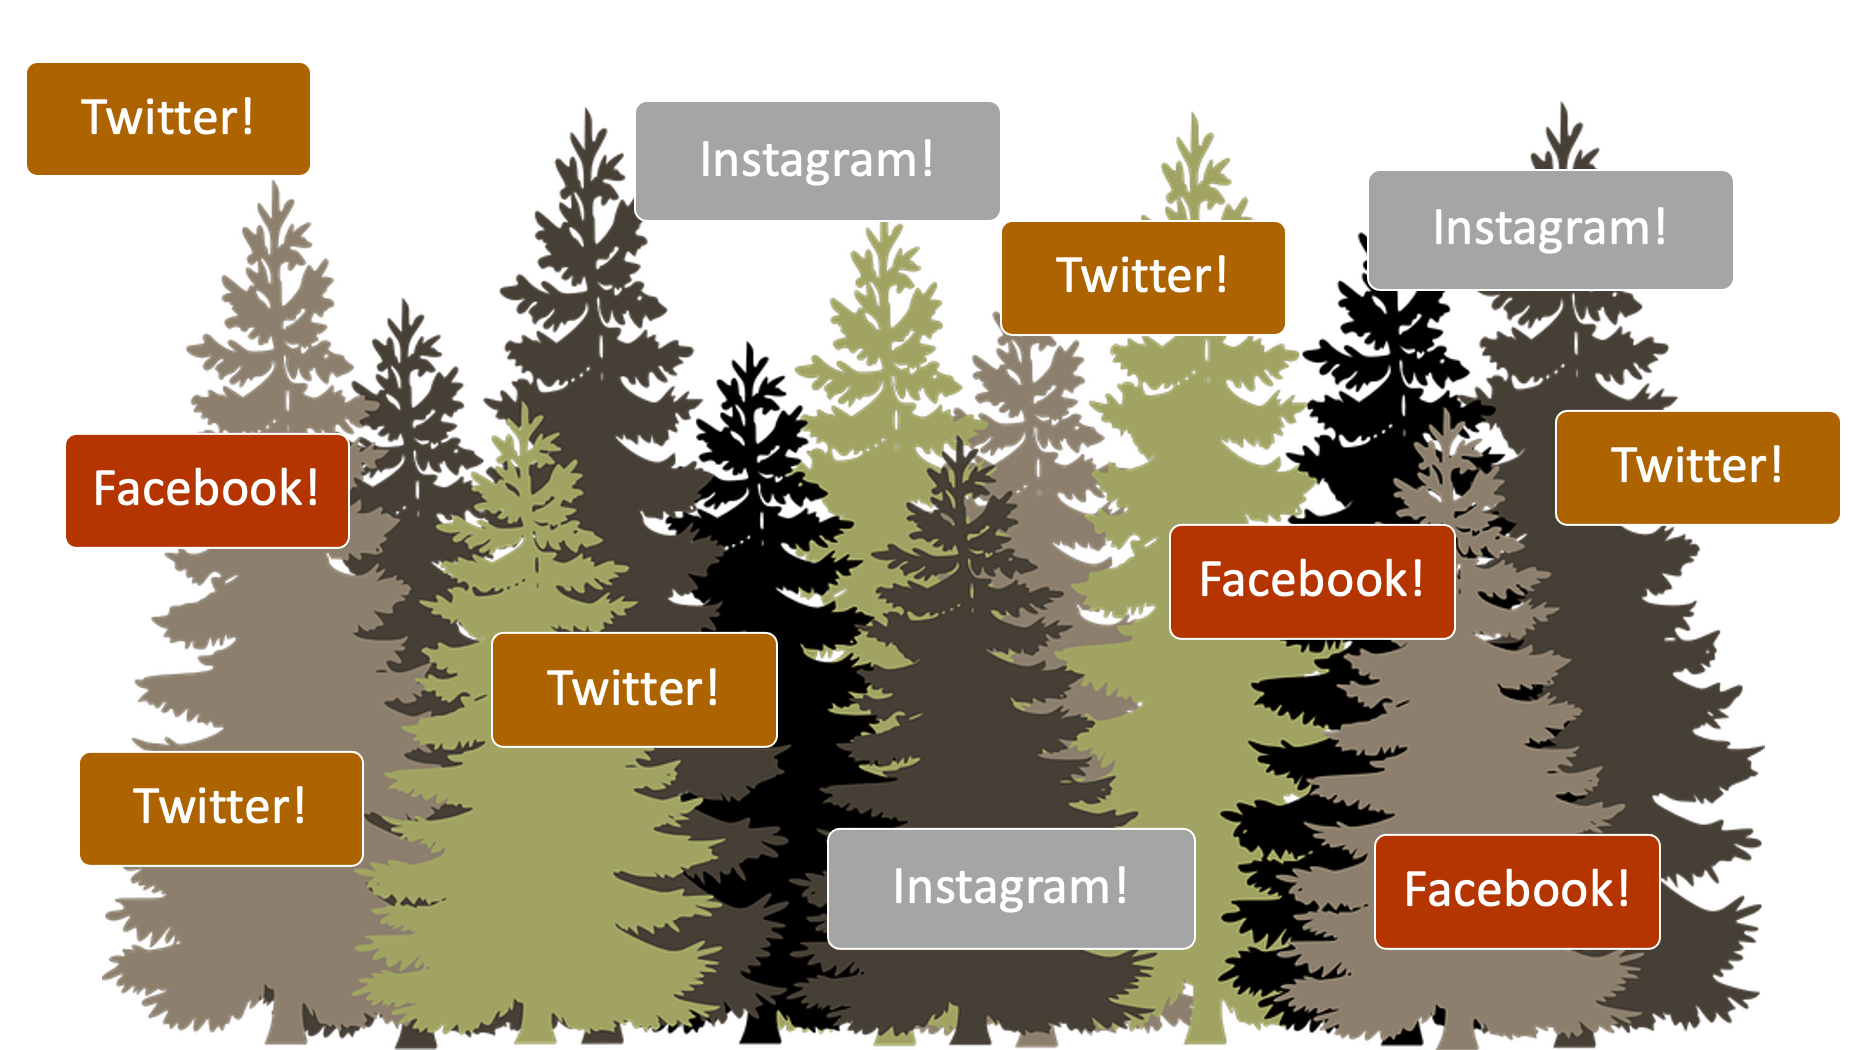
\includegraphics[width=\linewidth,height=\textheight,keepaspectratio]{../pictures/randomforest.png} \\\
	\end{center}
	

	
\end{frame}




\begin{frame}{Recap}
	
	Many different models available for machine learning.
	
	How do you know what is the best for your case? Try it out and validate!
	

\end{frame}



\begin{frame}{Zooming out} 
	
	We talked about:
	\begin{itemize}
		\item Rule-based Text Classification
		\item Automated Text Classification: SML
		\item The principles behind SML
		\item Some commonly used ML models \\\
	\end{itemize}
	
	Next, we will talk about:
	\begin{itemize}
		\item Validating models
	\end{itemize}
	
\end{frame}


\section{Validating models}


\begin{frame}{Precision and Recall}
	
	Precision quantifies the number of positive class predictions that actually belong to the positive cases. \\\ 
	OR: How much of what we found is actually correct?
	
	Recall quantifies the number of positive class prediction made out of all positive examples in the dataset. \\\
	OR: How many of the cases that we wanted to find did we actually find?
	

	
\end{frame}



\begin{frame}{Precision and Recall}
	
	\begin{center}
		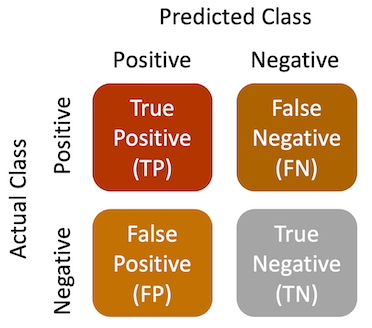
\includegraphics{../pictures/confusionmatrix_words.png} \\\
	\end{center}

	
	
\end{frame}


\begin{frame}{Precision and Recall} 
	
	\begin{columns}
		\column{.3\textwidth}
		\makebox[\columnwidth]{
			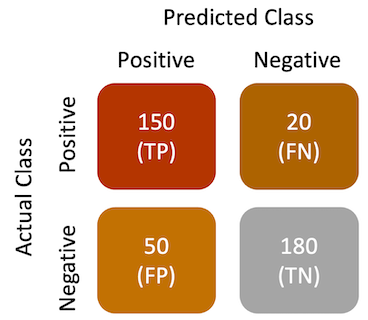
\includegraphics[width=\columnwidth,height=\paperheight,keepaspectratio]{../pictures/confusionmatrix_numbers.png}}
		\column{.7\textwidth}
		Precision is calculated as: \(\frac{\rm{TP}}{\rm{TP}+\rm{FP}}\) \\\
		In our case \(\frac{\rm{150}}{\rm{150}+\rm{50}}\) which is \(0.75\) \\\
		Recall is calculated as \(\frac{\rm{TP}}{\rm{TP}+\rm{FN}}\) \\\
		In our case \(\frac{\rm{150}}{\rm{150}+\rm{20}}\) which is \(0.88\)
	\end{columns}
	

	
\end{frame}


\begin{frame}[fragile]{What does this look like in code?}
	
A model based on a count vectorizer and Naïve Bayes:
	
\begin{lstlisting}
from sklearn.feature_extraction.text import (CountVectorizer)
from sklearn.naive_bayes import MultinomialNBB

countvectorizer = CountVectorizer(stop_words="english")
X_train = countvectorizer.fit_transform(texts_train)
X_test = countvectorizer.transform(texts_test)

nb = MultinomialNB()
nb.fit(X_train, labels_train)
y_pred = nb.predict(X_test)
\end{lstlisting}
	
\end{frame}





\begin{frame}[fragile]{What does this look like in code?}
	
Let's ask for a confusion matrix: 

\begin{lstlisting}
from sklearn.metrics import confusion_matrix

y_test = [0, 1, 1, 1, 0]
y_pred = [0, 0, 1, 1, 1]

print(confusion_matrix(y_test, y_pred))
\end{lstlisting}

\begin{lstlistingoutput}
[[1  1 ]
[ 1  2]]
\end{lstlistingoutput}
	
\end{frame}


\begin{frame}[fragile]{What does this look like in code?}
	
Let's get some metrics for validation: 
	
\begin{lstlisting}
from sklearn.metrics import classification_report
print(classification_report(y_test, y_pred))
\end{lstlisting}
	
\begin{lstlistingoutput}
              precision    recall  f1-score   support

0       0.50      0.50      0.50         2
1       0.67      0.67      0.67         3

accuracy                           0.60         5
macro avg       0.58      0.58      0.58         5
weighted avg       0.60      0.60      0.60         5
\end{lstlistingoutput}
	
\end{frame}


\begin{frame}{\(F_1\)-score}
	
	\(F_1\)-score: The harmonic mean of precision and recall. \\
	
	\(F_1\)-score \(= 2 \cdot \frac{\rm precision \cdot recall}{\rm precision + recall}\)
	

	
\end{frame}



\begin{frame}{Precision and Recall}
	
	\begin{center}
		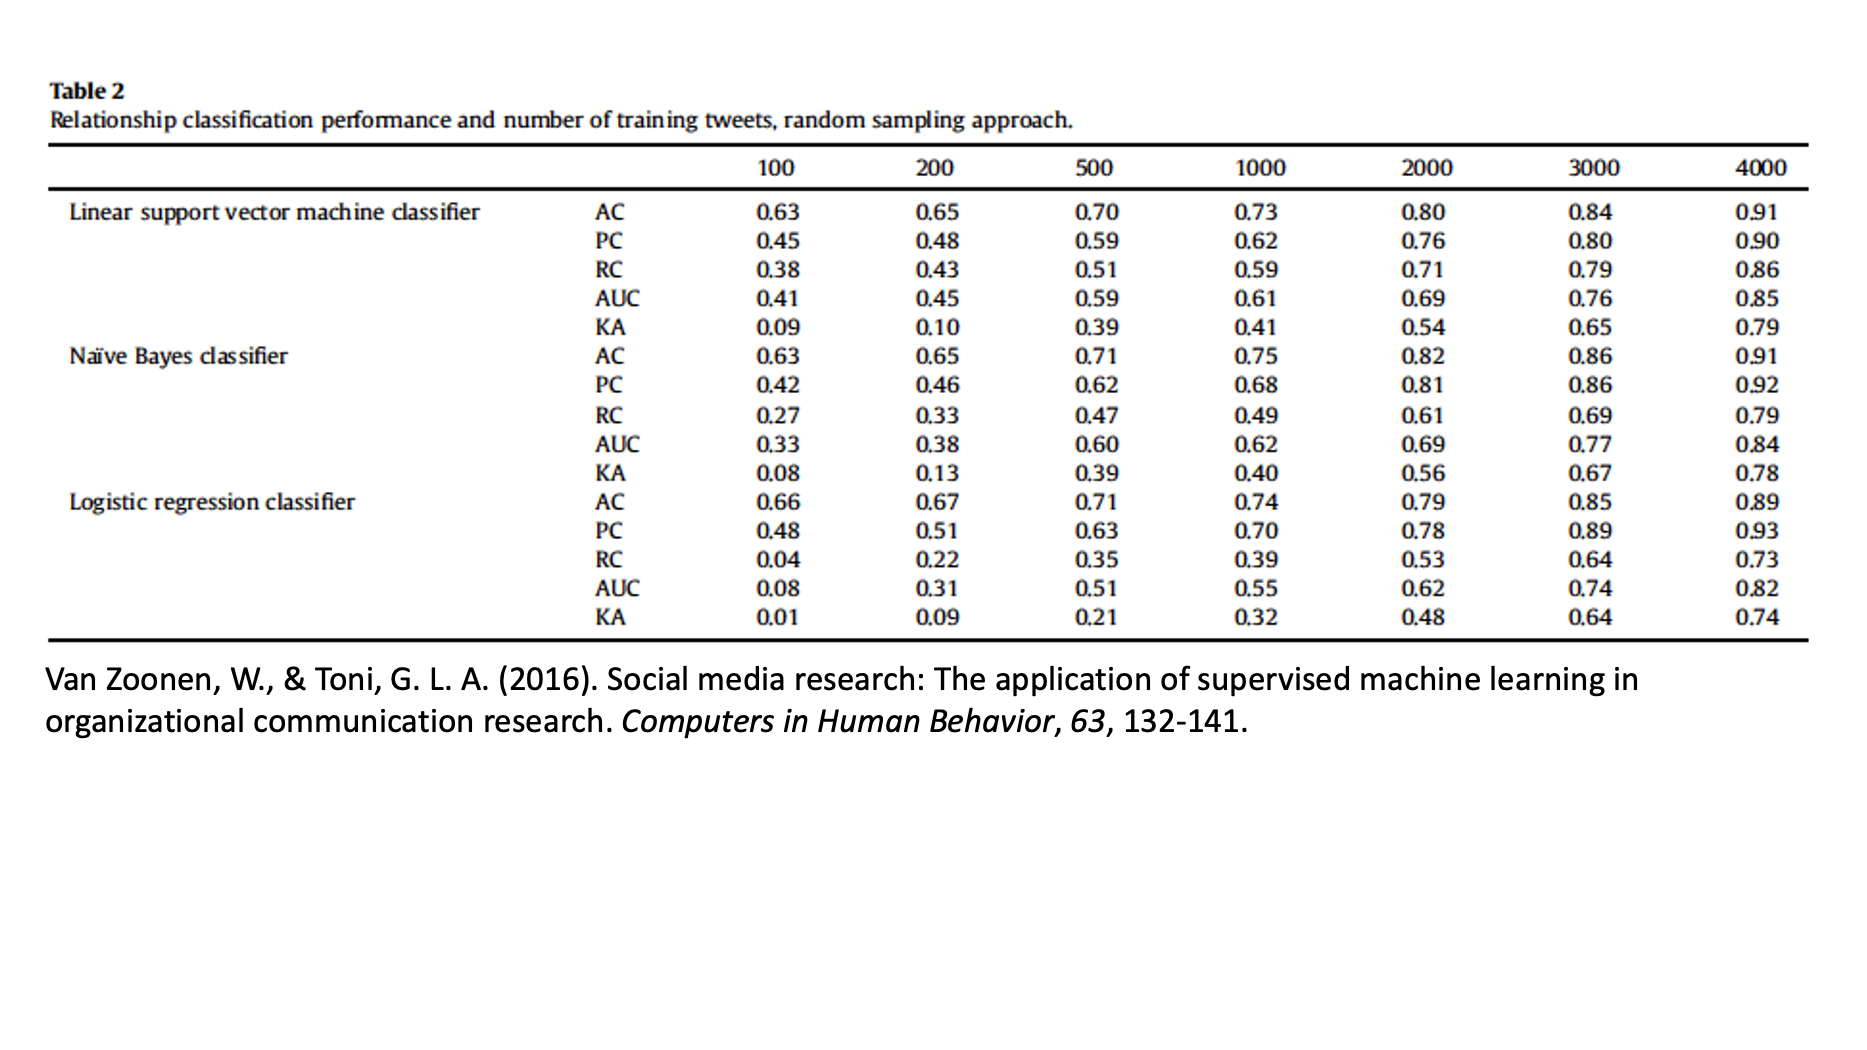
\includegraphics[width=\linewidth,height=\textheight,keepaspectratio]{../pictures/VanZoonen.png} \\\
	\end{center}
	
	\begin{tiny}
		\fullcite{van_zoonen_social_2016} 
	\end{tiny}
	

\end{frame}






\begin{frame}{Accuracy}
	
	Accuracy: In which percentage of all cases was our classifier right? \\
	
	Class distribution: The number of examples that belong to each class. \\
	
	Imbalanced classification: A classification predictive modeling problem where the distribution of examples across the classes within a training dataset is not equal.
	

	
\end{frame}


\begin{frame}{Accuracy}
	
	\begin{center}
		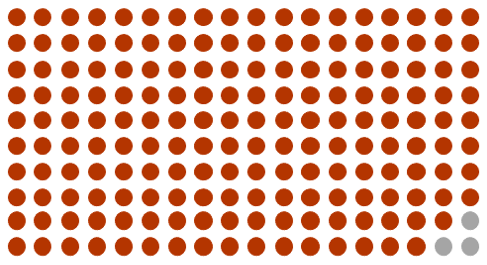
\includegraphics[width=\linewidth,height=\textheight,keepaspectratio]{../pictures/imbalance.png} 
	\end{center}	
	
	Majority class (red dots) vs. minority class (grey dots) 
	

\end{frame}



\begin{frame}{Validating Models}
	
	Many more metrics to validate models. \\
	
	Learn more using, for example, the scikit-learn documentation. 
	
\end{frame}



\begin{frame}{Zooming out} 
	
Today, we talked about:
\begin{itemize}
	\item Rule-based Text Classification
	\item Automated Text Classification: SML
	\item The principles behind SML
	\item The steps of SML
	\item Some commonly used ML models
	\item Validating models \\\
\end{itemize}


\end{frame}


\begin{frame}
	In this week's tutorial, you will:
\begin{itemize}
	\item Get some hands-on experience with supervised machine learning
	\item Discuss the first 5 questions of the tutorial exercise of week 8 \\\
\end{itemize}

To do:
\begin{itemize}
	\item Work on the first 5 questions of the tutorial exercise of week 8
\end{itemize}

\end{frame}



	
\end{document}